% IA 642 Defensive Security
% Week 03 Module 02 Lab: Harden and Instrument a Meridian Endpoint
% Submit as: Ali_Usama_Week03_Module02_Lab.pdf
\documentclass[11pt,letterpaper]{article}

\usepackage[margin=0.9in]{geometry}
\usepackage{array}
\usepackage{booktabs}
\usepackage{tabularx}
\usepackage{enumitem}
\usepackage{parskip}
\usepackage{ragged2e}
\usepackage{titlesec}
\usepackage{hanging}
\usepackage[colorlinks=true,linkcolor=blue,citecolor=blue,urlcolor=blue]{hyperref}
\usepackage{xurl}
\usepackage{graphicx}
\usepackage{float}
\usepackage{microtype}
\usepackage{xcolor}
\usepackage{colortbl}

\hypersetup{pdfauthor={Unais Ali; Hafiz Usama}, pdftitle={IA 642 Week 03 Lab 3.2 Meridian Endpoint}}

\definecolor{tblhead}{HTML}{1F4E79}
\definecolor{tblrow}{HTML}{F0F4F8}
\setlength{\parindent}{0pt}
\renewcommand{\arraystretch}{1.28}
\setlength{\tabcolsep}{4pt}
\newcommand{\labtablesetup}{%
  \small
  \setlength{\tabcolsep}{6pt}%
  \renewcommand{\arraystretch}{1.45}%
}
\raggedbottom
\setlist[itemize]{leftmargin=1.2em,itemsep=0.25em,topsep=0.35em,parsep=0pt}
\setlist[enumerate]{leftmargin=1.3em,itemsep=0.35em,topsep=0.35em,parsep=0pt}
\newcolumntype{Y}{>{\RaggedRight\arraybackslash}X}
\newcolumntype{L}[1]{>{\RaggedRight\arraybackslash}p{#1}}
\titleformat{name=\section,numberless}{\large\bfseries\color{tblhead}}{}{0em}{}
\titlespacing*{name=\section,numberless}{0pt}{1.1em}{0.4em}
\titleformat{name=\subsection,numberless}{\normalsize\bfseries\color{tblhead}}{}{0em}{}
\titlespacing*{name=\subsection,numberless}{0pt}{0.8em}{0.28em}

\newcommand{\aparef}[2]{\hyperref[ref:#1]{#2}}
\newcommand{\refitem}[1]{\phantomsection\label{ref:#1}}

\begin{document}

\begin{center}
{\large\textbf{EASTERN MICHIGAN UNIVERSITY}}\\[0.12em]
{\normalsize College of Engineering and Technology}\\[0.25em]
{\Large\textbf{IA 642: Defensive Security}}\\[0.15em]
{\large\textbf{Week 03, Module 02 Lab: Harden and Instrument a Meridian Endpoint}}\\[0.2em]
{\small Endpoint Defense \& Detection \quad\textbullet\quad NUR-CLIN-014 Rebuild}
\end{center}

\vspace{0.35em}\hrule\vspace{0.45em}

\begin{tabularx}{\textwidth}{@{}L{3.2cm}Y L{2.0cm}Y@{}}
\textbf{Group members} & Unais Ali & \textbf{EID} & E02805019 \\
 & Hafiz Usama &  & E02574092 \\
\textbf{Course} & IA 642 Defensive Security & \textbf{Week} & 3, Lab 3.2 \\
\textbf{Host} & NUR-CLIN-014 (cardiology nurse station) & \textbf{Date} & September 2026 \\
\end{tabularx}

\vspace{0.35em}
\textit{Meridian Health Network continues from Lab~2.3 (network boundaries / infusion-pump segmentation). This lab goes inside one of those zones, hardens the rebuilt clinical workstation NUR-CLIN-014, and writes Endpoint Detection and Response (EDR) detections for the attacker behaviors recovered from the old build. It is separate from the Week~02 university payment TARA case.}

\section*{1. Part A: Fork and Baseline}

\begingroup\labtablesetup
\rowcolors{2}{white}{tblrow}
\begin{tabularx}{\textwidth}{@{}L{3.4cm}Y@{}}
\toprule
\rowcolor{tblhead}
\textcolor{white}{\textbf{Question}} & \textcolor{white}{\textbf{Answer}} \\
\midrule
\rowcolor{white}
Fork & \textbf{Windows} (Windows 11 Enterprise workstation image for shared nurse-station use). \\
Published baseline & \textbf{CIS Microsoft Windows 11 Enterprise Benchmark}, Level~1 (Workstation profile), current release used by Meridian imaging. \\
Why this baseline & Meridian is a civilian healthcare provider, not a DoD system, so a CIS Level~1 workstation profile matches the EHR/imaging/e-prescribing role without importing STIG operational cost that clinical 24/7 shared stations cannot absorb. \\
Application-control mechanism & \textbf{WDAC} (AppLocker retained only as a legacy audit path during cutover). \\
\bottomrule
\end{tabularx}
\endgroup

\noindent The lecture's five control goals are the same on every OS; only the mechanisms change. Figure~\ref{fig:osarch} places Windows and Linux side by side. NUR-CLIN-014 answers the \textbf{Windows} column (WDAC, Credential Guard / LSASS, NTFS ACLs, least-privilege services, CIS Windows 11 Enterprise L1). SELinux / AppArmor would apply only if Meridian had forked Linux.

\noindent\textbf{NIST SP~800-53 mapping (why this endpoint program exists).}
This lab covers the three families named in the module slide:

\begingroup\labtablesetup
\rowcolors{2}{white}{tblrow}
\begin{tabularx}{\textwidth}{@{}>{\RaggedRight\arraybackslash}p{1.1cm} >{\RaggedRight\arraybackslash}p{2.5cm} >{\RaggedRight\arraybackslash}X@{}}
\toprule
\rowcolor{tblhead}
\textcolor{white}{\textbf{Control}} &
\textcolor{white}{\textbf{Family}} &
\textcolor{white}{\textbf{How NUR-CLIN-014 answers it}} \\
\midrule
\rowcolor{white}
CM-6 & Configuration Settings
  & CIS Windows~11 Enterprise Level~1 hardening baseline + Part~B control table (WDAC, Credential Guard, NTFS ACLs, service identities, logging). \\
SI-3 & Malicious Code Protection
  & WDAC allowlisting plus EDR response actions that block or alert on unauthorized execution (Run-key implants, side-loaded DLLs, LOLBAS downloaders). \\
SI-4 & System Monitoring
  & Part~D detection logic: Sysmon/EDR telemetry, ATT\&CK-mapped rules, LSASS ProcessAccess detection, and Part~E sensor heartbeat so monitoring does not go silent. \\
\bottomrule
\end{tabularx}
\endgroup

\begin{figure}[H]
\centering
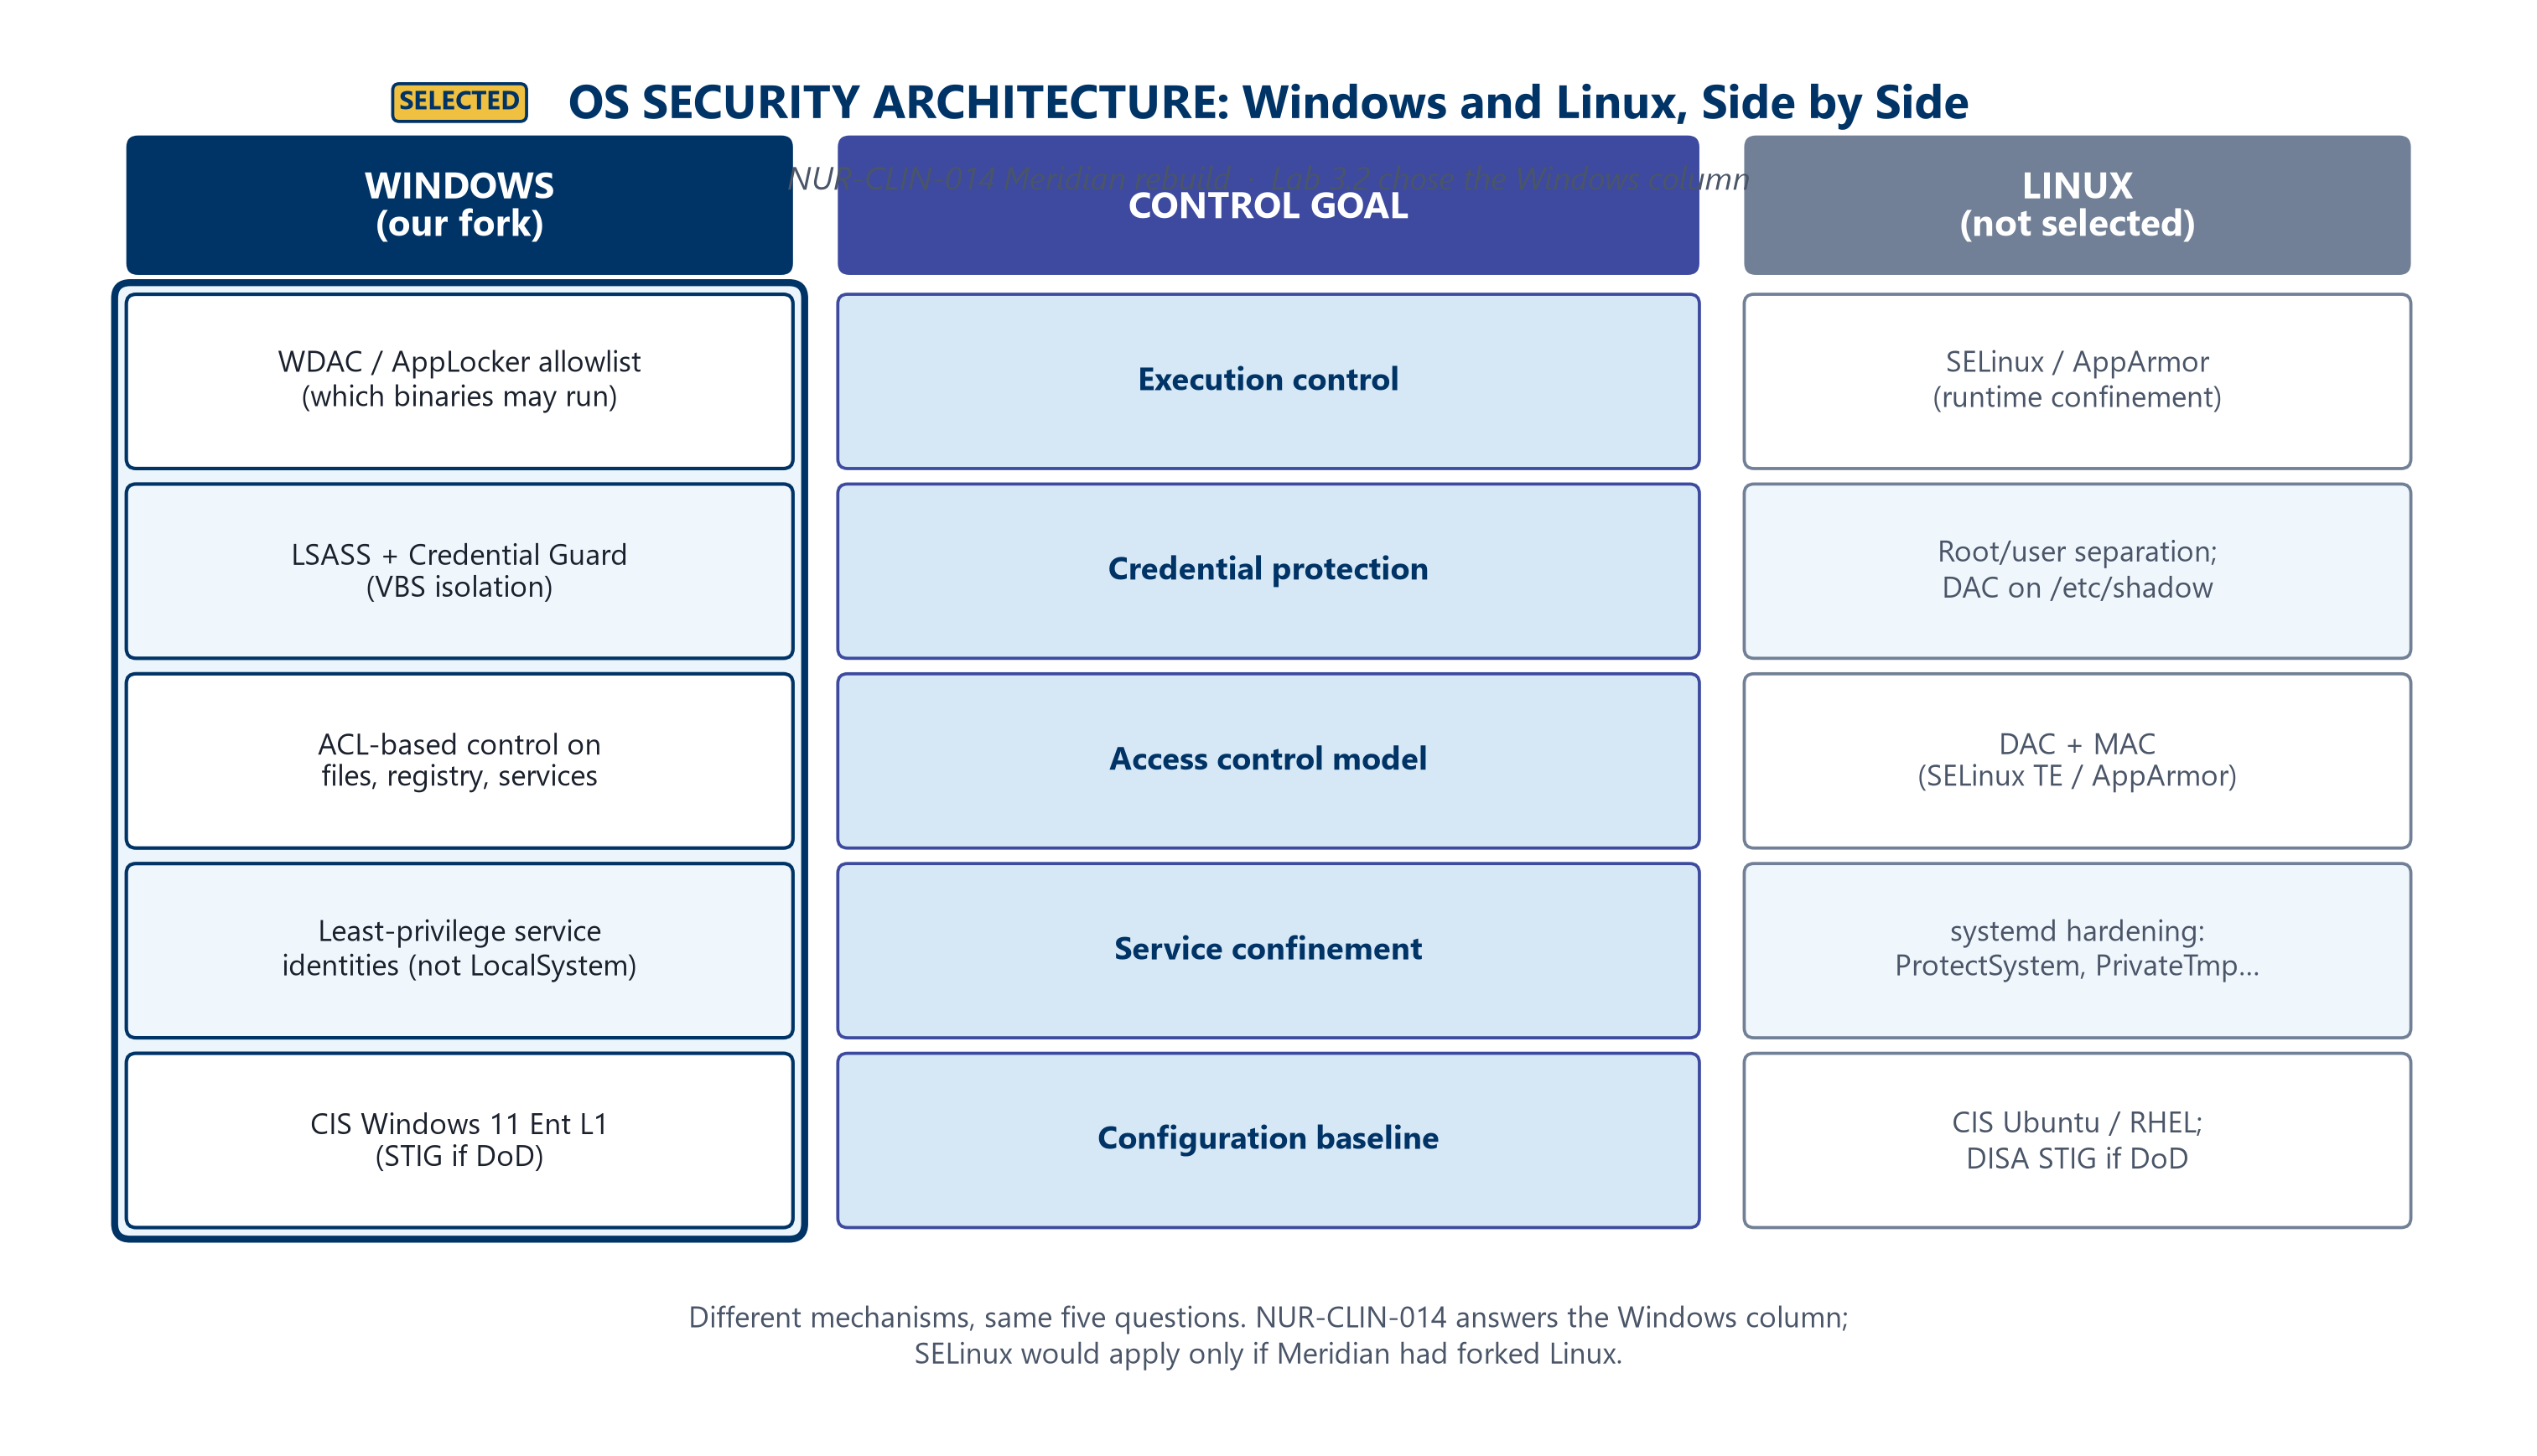
\includegraphics[width=0.98\textwidth]{figures/fig_os_architecture.png}
\caption{Author-created Windows vs.\ Linux security-architecture map for Meridian NUR-CLIN-014. Same five control goals as the course Figure~2 slide; this rebuild uses the Windows mechanisms.}
\label{fig:osarch}
\end{figure}

\begin{figure}[H]
\centering
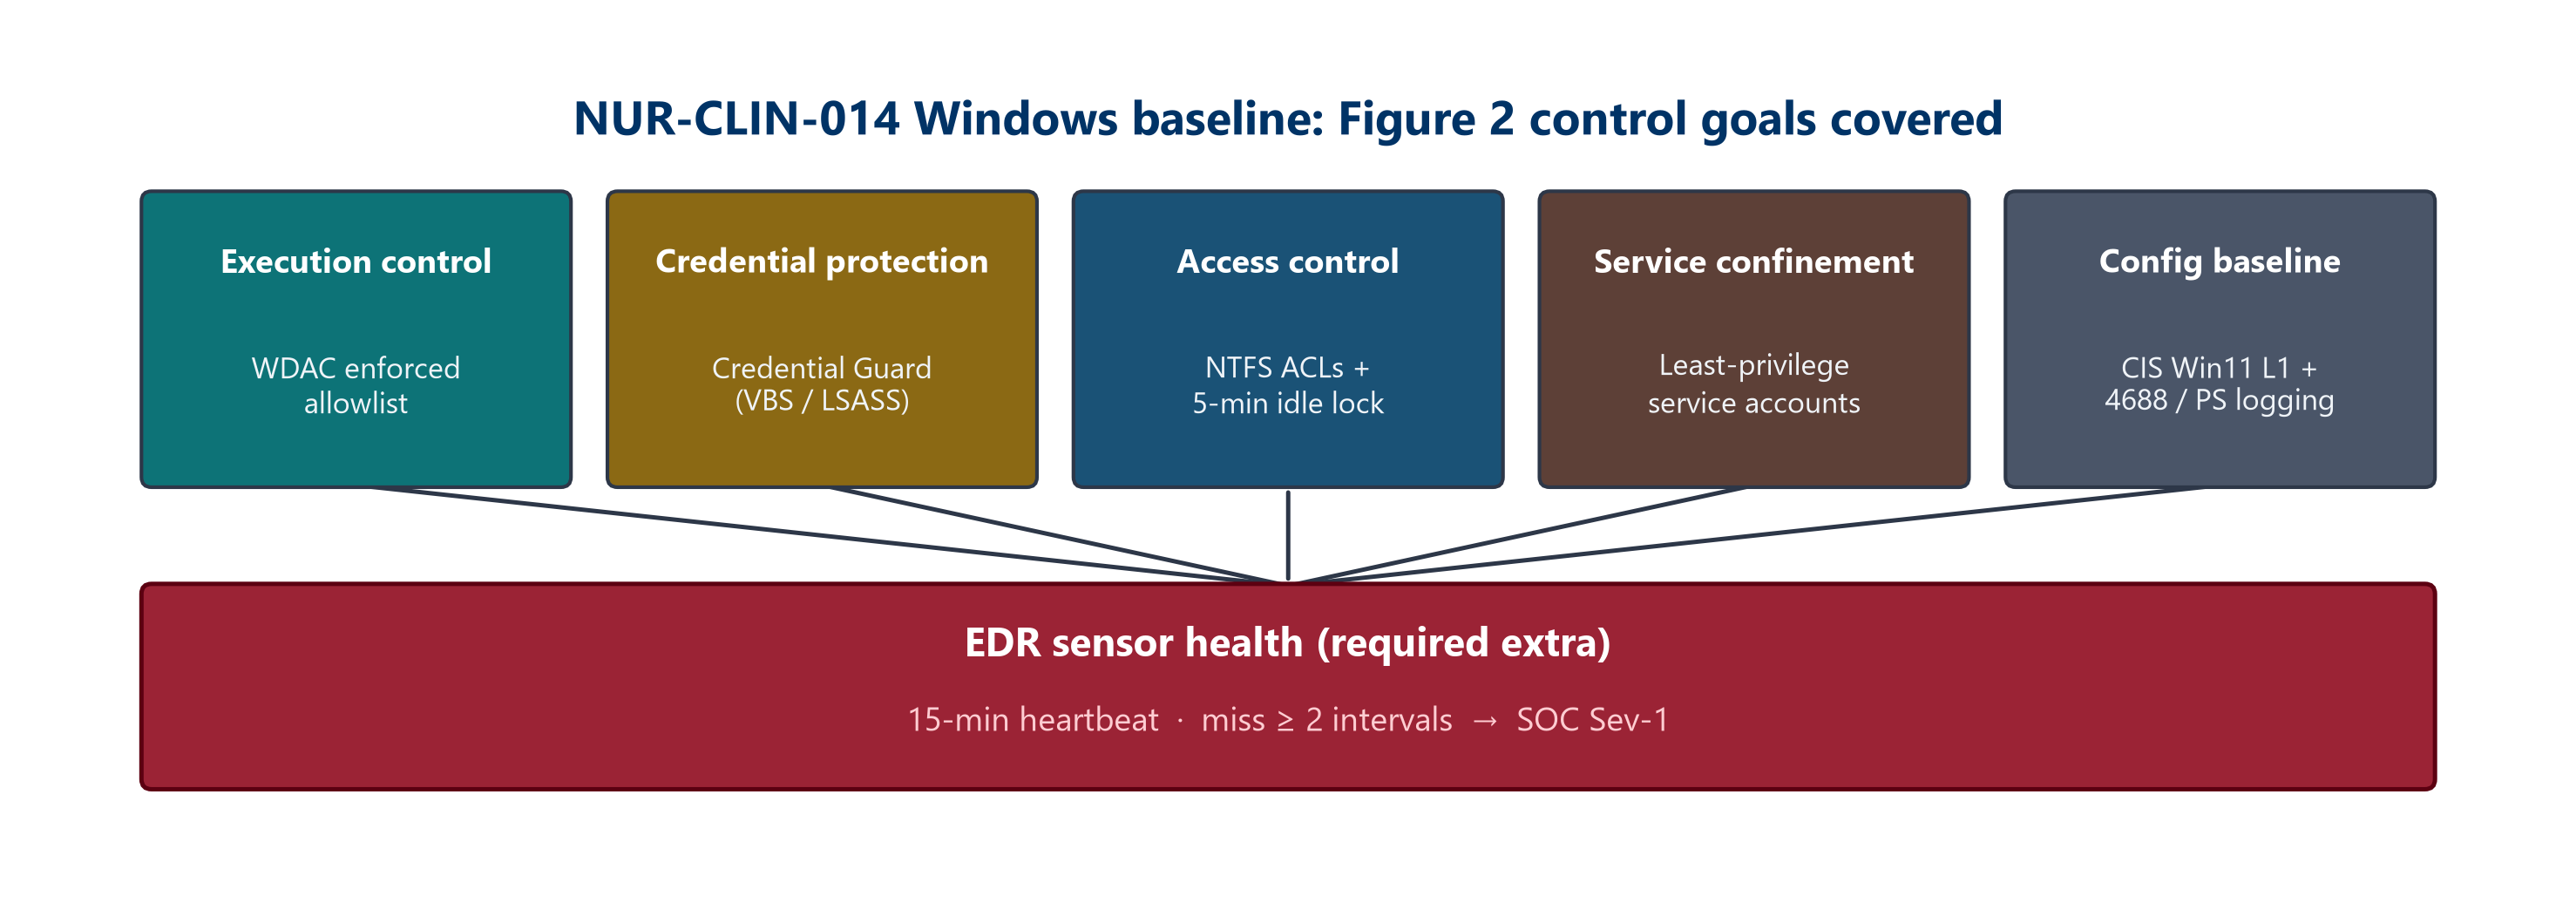
\includegraphics[width=0.95\textwidth]{figures/fig_control_goals.png}
\caption{Author-created map of how the NUR-CLIN-014 Windows baseline answers each Figure~2 control goal, plus the required EDR sensor-health control.}
\label{fig:goals}
\end{figure}

\noindent Hardening alone is not enough. Figure~\ref{fig:stack} is Meridian's seven-layer endpoint defense stack for this rebuild: Layers~1--5 harden (baseline, privilege, Credential Guard, WDAC, service confinement); Layers~6--7 detect and respond (EDR telemetry + sensor health, isolate/kill/reimage). An attacker must defeat every layer \emph{and} stay invisible to the last two.

\begin{figure}[H]
\centering
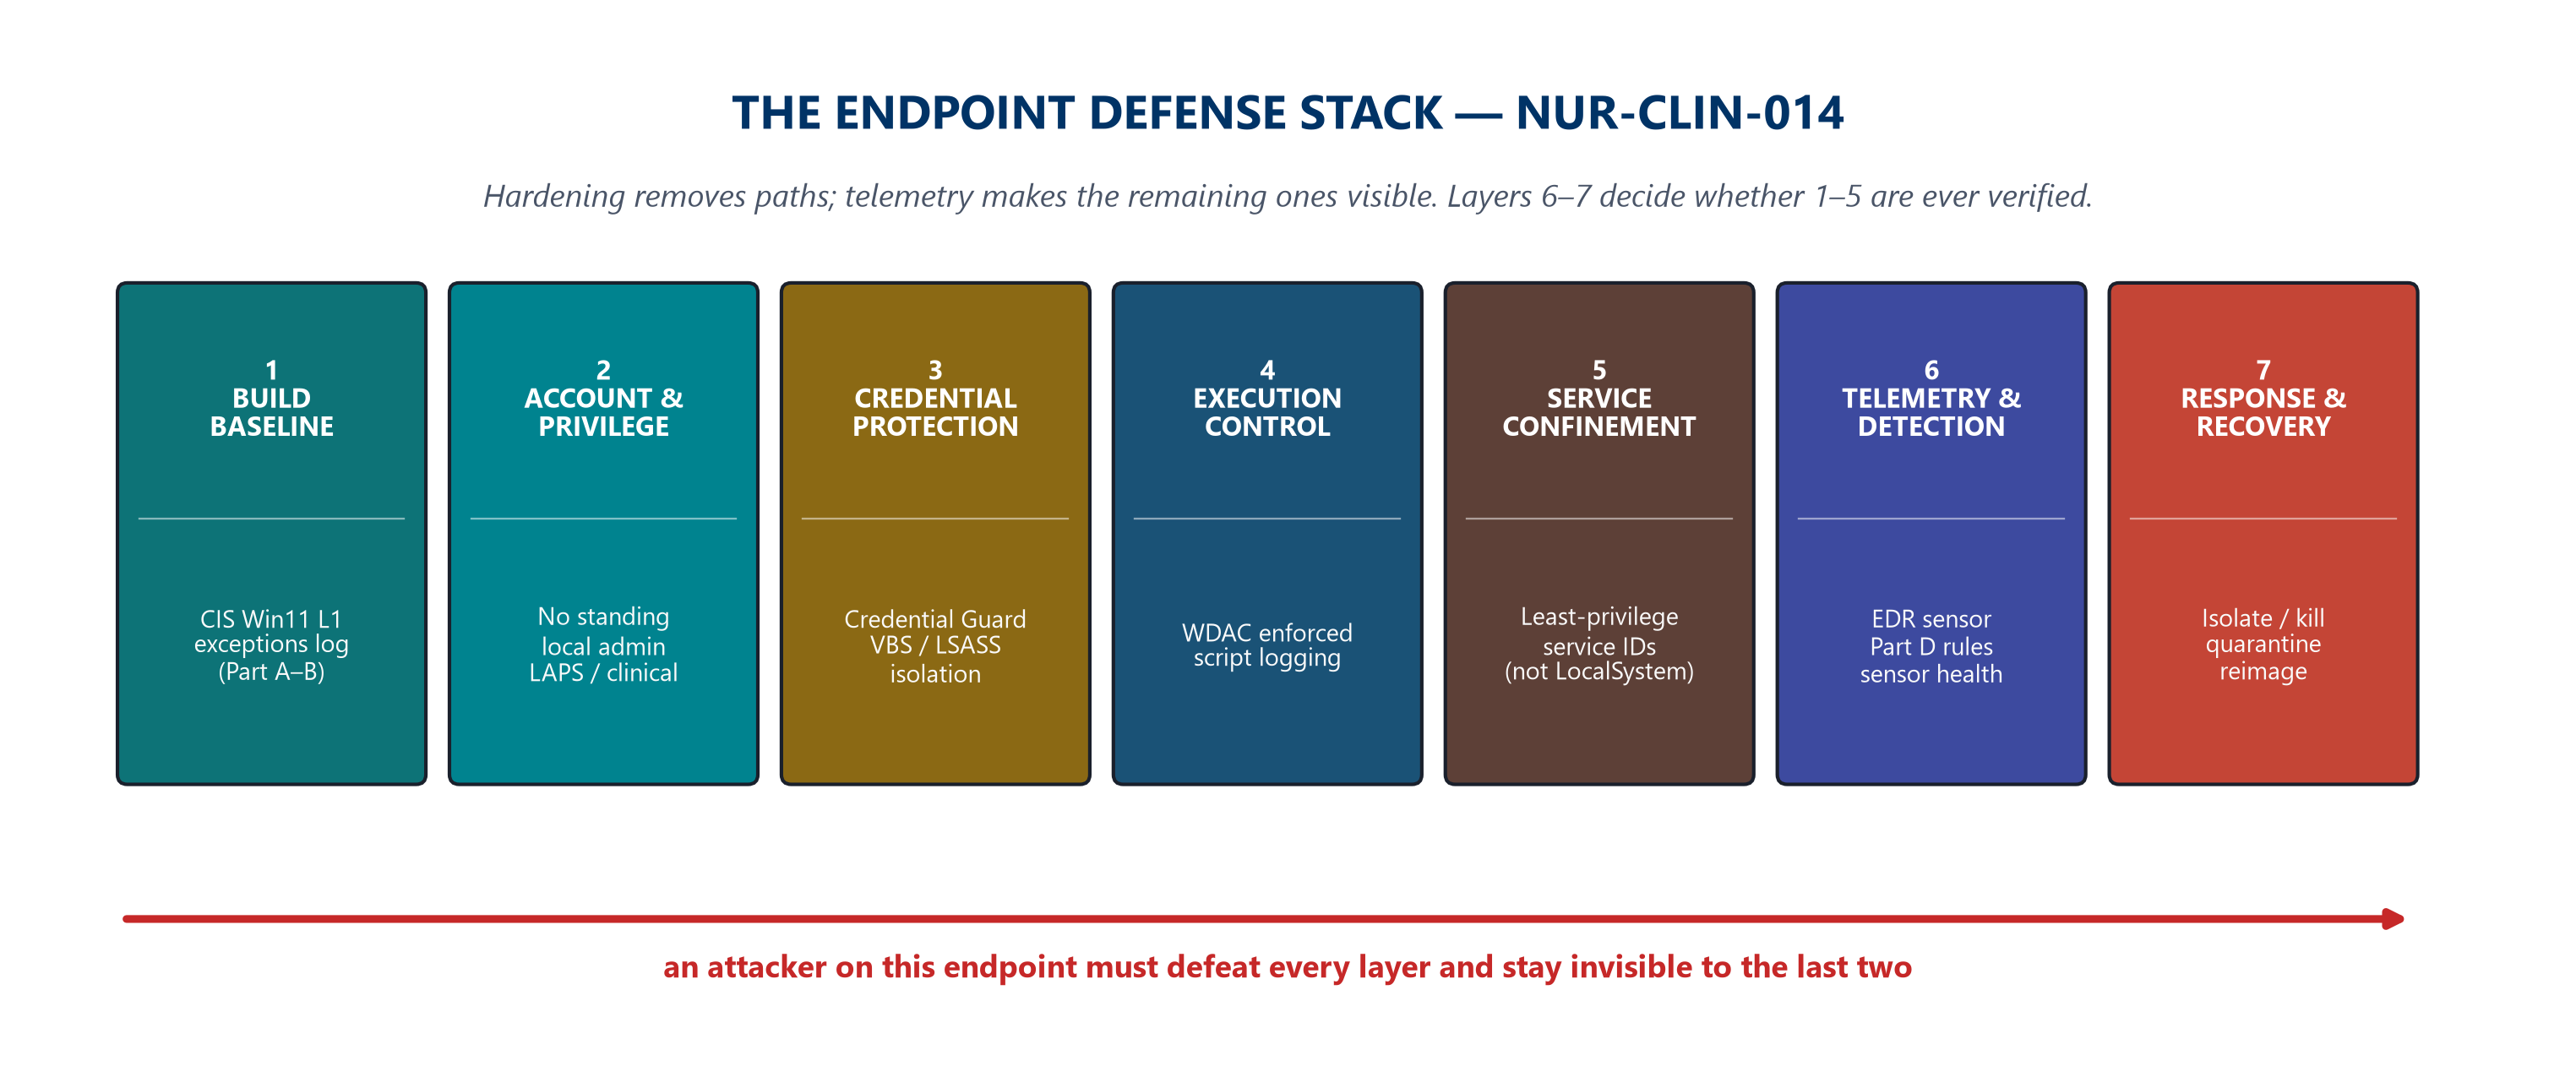
\includegraphics[width=0.98\textwidth]{figures/fig_defense_stack.png}
\caption{Author-created endpoint defense stack for NUR-CLIN-014, mapped to Lab~3.2 Parts A--E. Hardening removes paths; telemetry verifies the rest.}
\label{fig:stack}
\end{figure}

\section*{2. Part B: Hardening Baseline}

\noindent A baseline applied once and never re-measured is a historical document. Figure~\ref{fig:lifecycle} is Meridian's lifecycle for NUR-CLIN-014: this lab deliverable completes \textbf{Select \& Scope} (Part~A) and \textbf{Tailor \& Document} (Step~3 exception log); Apply / Measure / Remediate Drift are the scheduled operations model after the rebuild image is signed.

\begin{figure}[H]
\centering
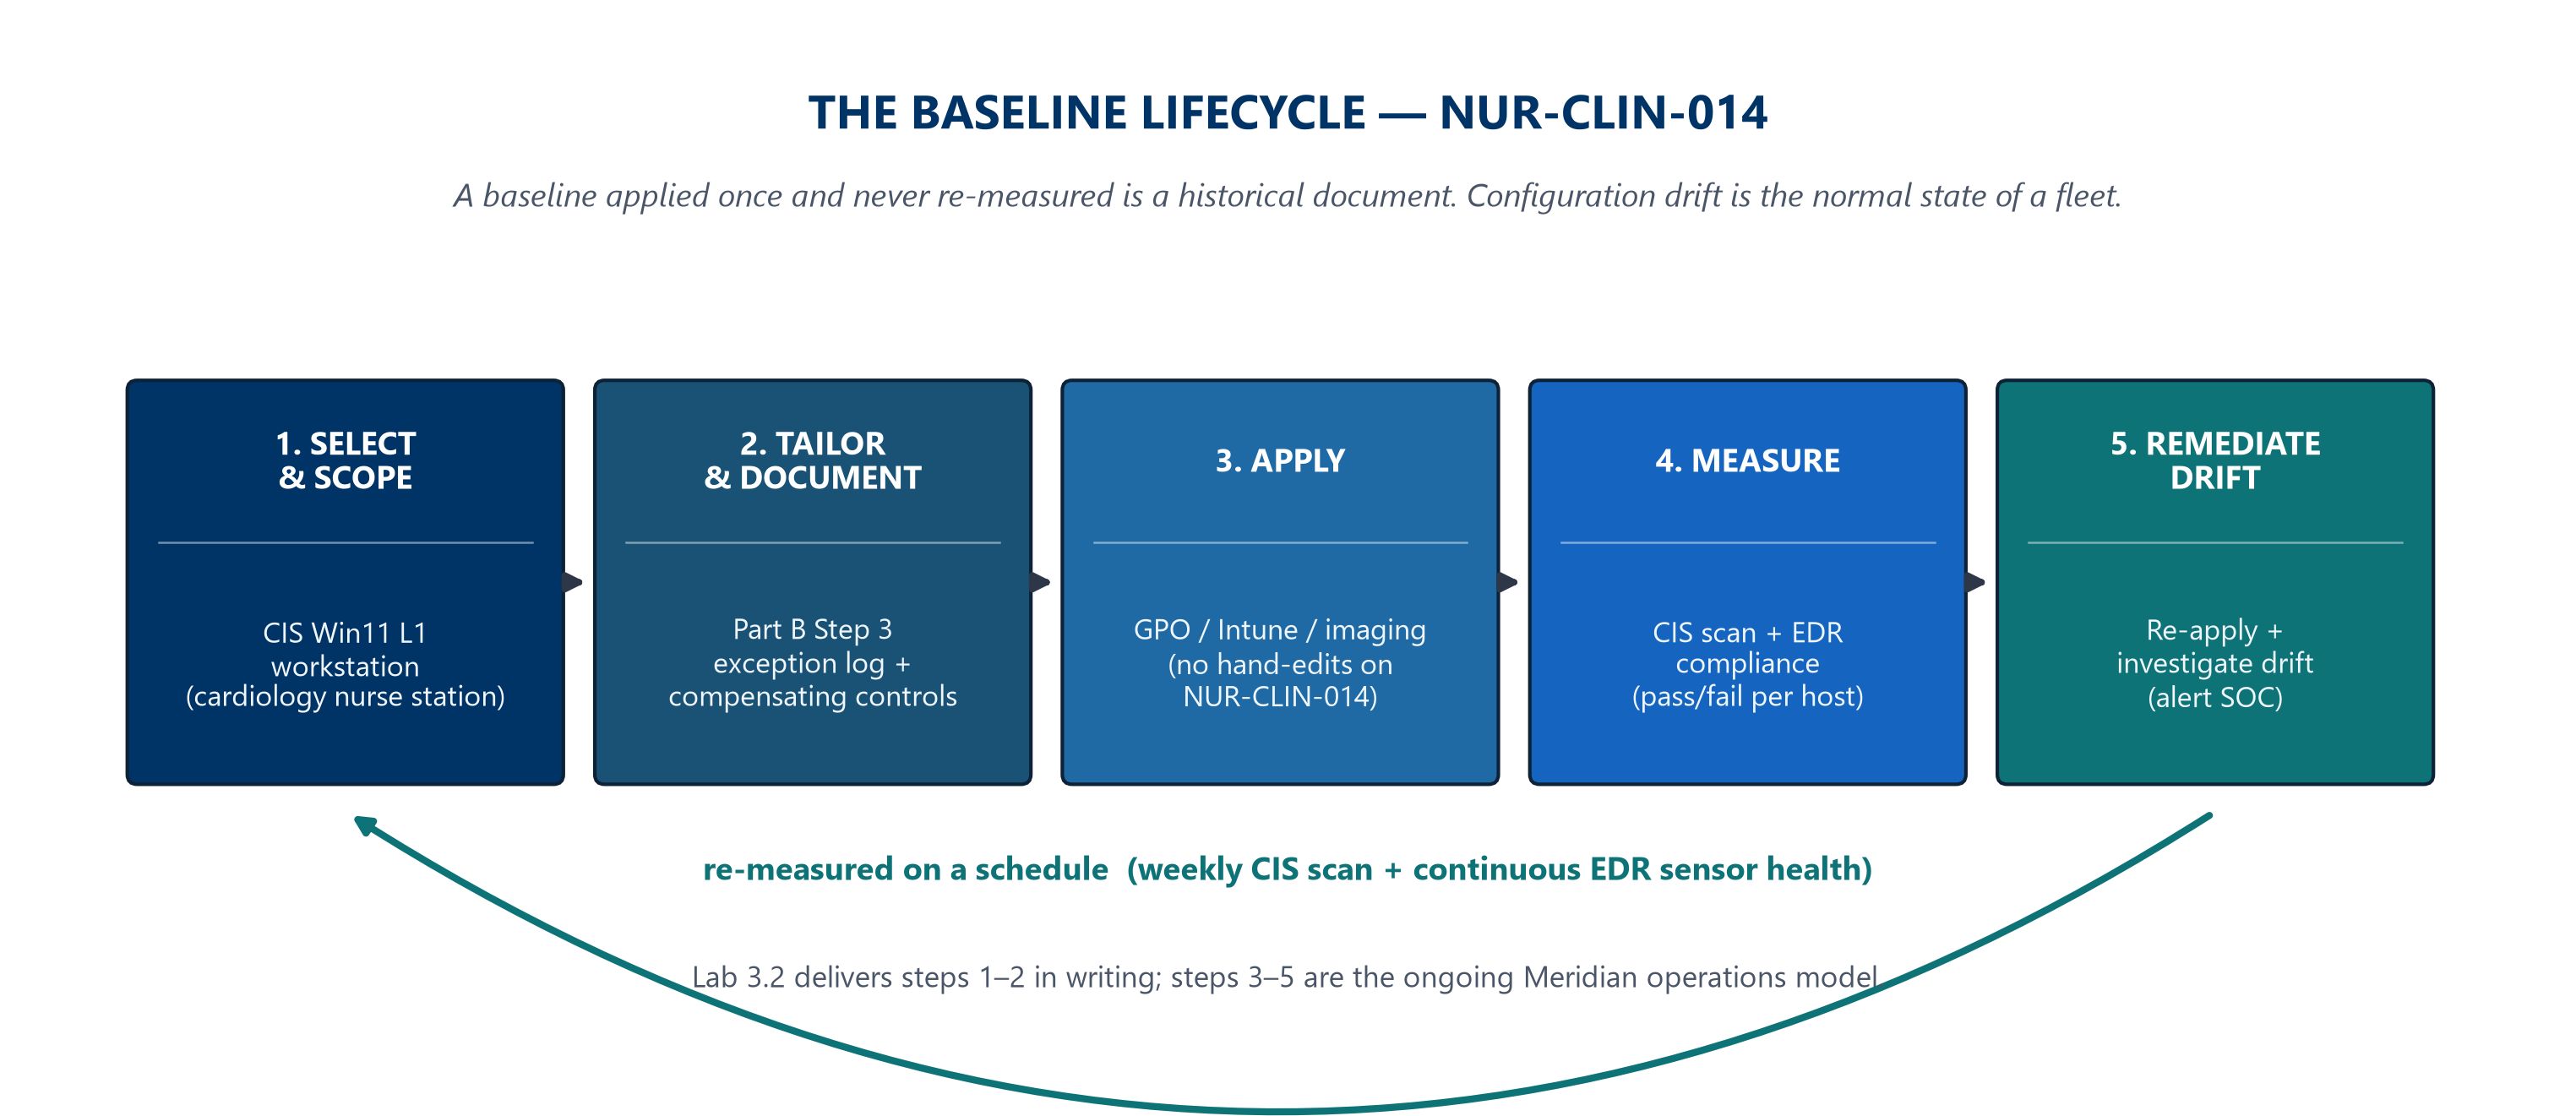
\includegraphics[width=0.98\textwidth]{figures/fig_baseline_lifecycle.png}
\caption{Author-created baseline lifecycle for NUR-CLIN-014, adapted from the course hardening-baselines slide. Drift is treated as a possible intrusion, not only misconfiguration.}
\label{fig:lifecycle}
\end{figure}

\subsection*{Step 2: Baseline control table}
At least one control addresses each Figure~2 goal (execution control, credential protection, access control, service confinement, configuration baseline) plus EDR sensor health (Figure~\ref{fig:goals}). The lab handout's worked Administrators-group example is \textbf{not} reused as one of these rows. Credential protection centers on isolating LSASS secrets with Credential Guard (built on VBS).

\begingroup\labtablesetup
\rowcolors{2}{white}{tblrow}
\begin{tabularx}{\textwidth}{@{}>{\bfseries\centering\arraybackslash}p{0.55cm} >{\RaggedRight\arraybackslash}p{2.35cm} >{\RaggedRight\arraybackslash}X >{\RaggedRight\arraybackslash}p{2.05cm} >{\RaggedRight\arraybackslash}X@{}}
\toprule
\rowcolor{tblhead}
\textcolor{white}{\textbf{\#}} &
\textcolor{white}{\textbf{Setting / Control}} &
\textcolor{white}{\textbf{Value}} &
\textcolor{white}{\textbf{Control Goal}} &
\textcolor{white}{\textbf{Risk It Closes}} \\
\midrule
\rowcolor{white}
1 & WDAC Code Integrity policy (enforced)
  & Allow only Microsoft-signed OS binaries, Meridian-signed clinical packages (EHR, imaging viewer, e-prescribing), and approved browser; deny user-writable paths
  & Execution control
  & Blocks unsigned payloads launched from temp directories (as seen via the old Run-key implant). \\
2 & Credential Guard (VBS isolation of LSASS)
  & Enabled; require UEFI Secure Boot + virtualization support on the rebuild image so LSASS credential material runs in a protected enclave
  & Credential protection
  & Stops reusable LSASS secrets from being dumped into attacker memory for lateral movement (the credential-dump path from the old build). \\
3 & NTFS ACLs on clinical application folders (\texttt{C:\textbackslash Program Files\textbackslash Meridian\textbackslash*})
  & Clinical users: Read \& execute only; Modify/Write denied; SYSTEM + named workstation-admins: Full control
  & Access control model
  & Stops a standard nurse account from replacing EHR/imaging binaries or dropping side-load DLLs beside trusted apps. \\
4 & Service account identity for vendor helpers
  & No clinical service runs as LocalSystem unless vendor-documented; otherwise dedicated gMSA / least-privilege service account
  & Service confinement
  & Limits blast radius if a helper service is abused for persistence (T1543-class installs). \\
5 & PowerShell / script logging
  & Module Logging, Script Block Logging, and Transcription enabled; Constrained Language Mode for standard users
  & Configuration baseline (CIS logging)
  & Makes living-off-the-land script staging visible to EDR instead of invisible. \\
6 & Process Creation auditing (4688) + command-line
  & Audit Process Creation success enabled; ``Include command line in process creation events'' = Enabled
  & Configuration baseline
  & Supplies command-line telemetry required by Part~D detections for tasks, services, and LOLBAS. \\
7 & Interactive logon: machine inactivity limit
  & 5-minute idle lock; unlock requires badge/PIN re-auth for shared station
  & Access control
  & Reduces corridor walk-up session hijack on a semi-public nurse station. \\
8 & EDR sensor health / heartbeat policy
  & Sensor must check in every 15 minutes; miss $\geq$ 2 intervals = critical ticket to SOC Tier~1
  & EDR sensor health
  & Prevents another 41-day silent-agent window like NUR-CLIN-014. \\
9 & Windows Security event log retention
  & Security log $\geq$ 1\,GB, retain as needed; clearing Security log generates high-severity SIEM alert
  & Configuration baseline / defense visibility
  & Makes T1070.001 log-clearing immediately visible instead of erasing evidence. \\
\bottomrule
\end{tabularx}
\endgroup

\subsection*{Step 3: Exception log}

\begingroup\labtablesetup
\rowcolors{2}{white}{tblrow}
\begin{tabularx}{\textwidth}{@{}>{\RaggedRight\arraybackslash}p{3.2cm} >{\RaggedRight\arraybackslash}p{3.4cm} >{\RaggedRight\arraybackslash}X@{}}
\toprule
\rowcolor{tblhead}
\textcolor{white}{\textbf{Baseline Item Not Applied}} &
\textcolor{white}{\textbf{Operational Reason}} &
\textcolor{white}{\textbf{Compensating Control}} \\
\midrule
Full WDAC block of the cardiology imaging viewer when it loads vendor plug-in DLLs outside the default Microsoft catalog
  & Vendor states the viewer fails under a pure Microsoft-only allowlist; cardiology cannot wait on IT mid-encounter
  & Publisher/hash allowlist limited to the signed vendor package path; EDR alert on any load of that viewer from a non-standard parent or from a user-writable directory. \\
Disabling the browser entirely (CIS ``remove unnecessary browsers'' style guidance)
  & E-prescribing and selected EHR workflows require an approved Chromium-based browser
  & WDAC allows only the managed browser binary; URL category filtering + SmartScreen; Extension allowlist enforced by GPO. \\
CIS guidance to remove local admin accounts entirely from the host
  & Break/fix imaging and overnight vendor patches sometimes require a controlled local elevation when domain Controllers are unreachable
  & LAPS rotates the single local admin password every 24 hours; all elevations logged and ticketed; no standing clinical users in Administrators. \\
\bottomrule
\end{tabularx}
\endgroup

\section*{3. Part C: ATT\&CK Mapping}

\begin{figure}[H]
\centering
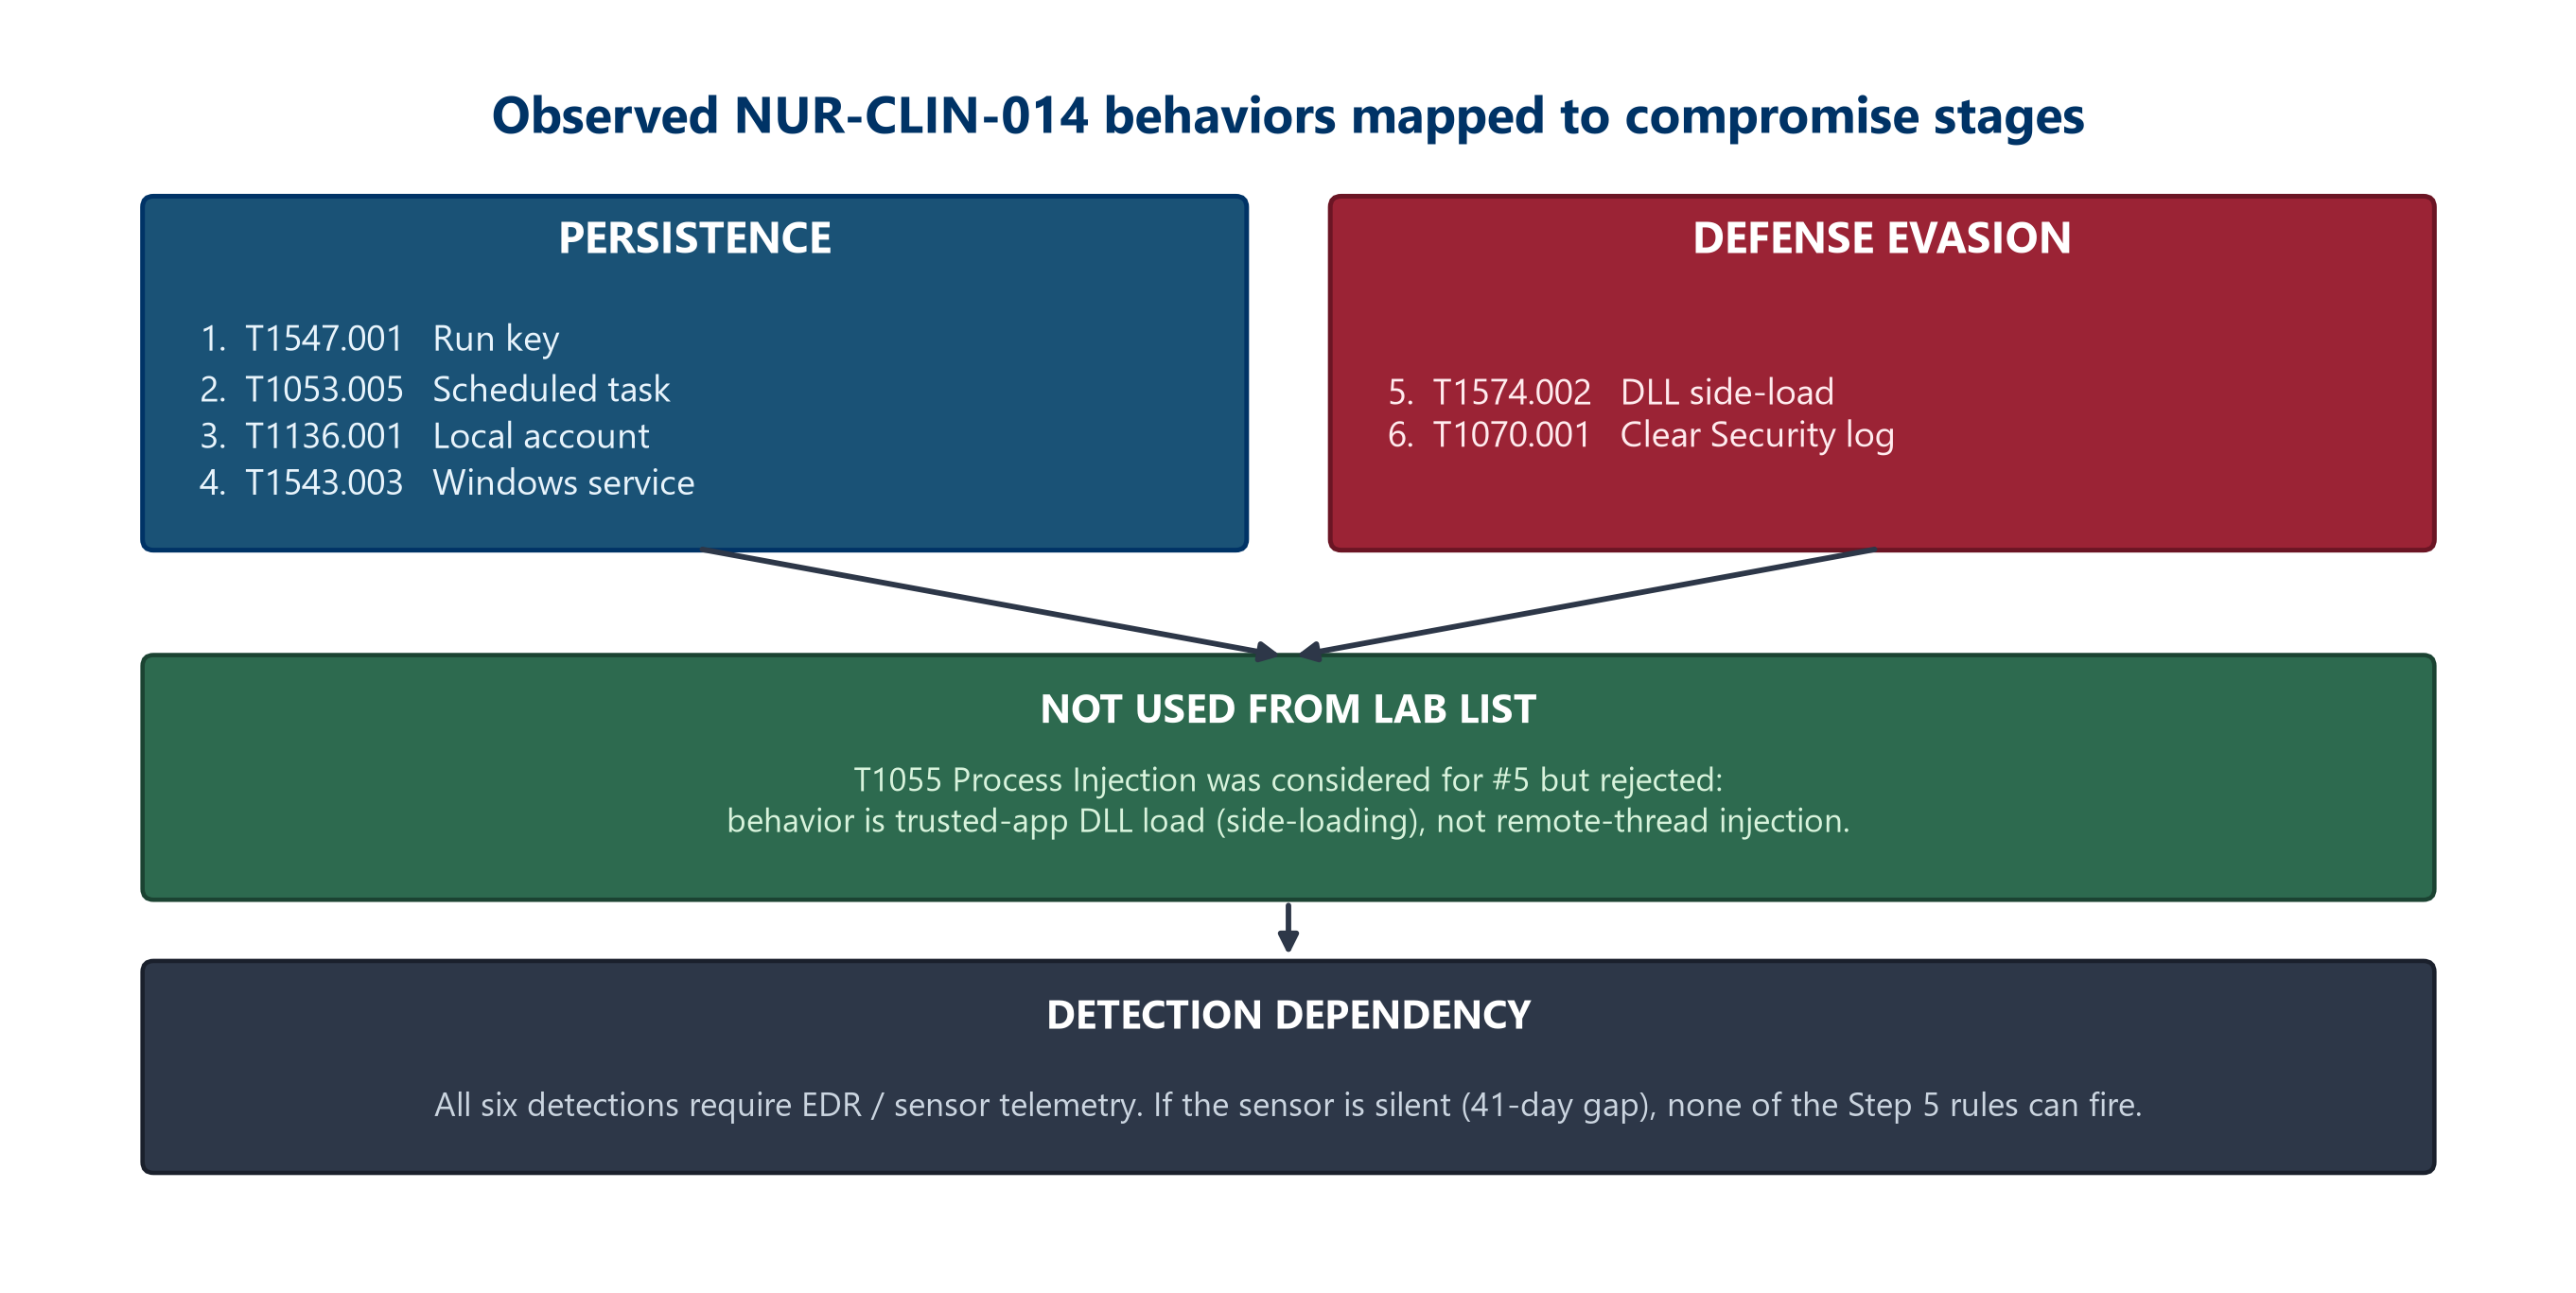
\includegraphics[width=0.92\textwidth]{figures/fig_attack_stages.png}
\caption{Author-created stage map for the six recovered behaviors. MITRE ATT\&CK technique T1055 was considered for behavior~5 and rejected in favor of T1574.002.}
\label{fig:stages}
\end{figure}

\begingroup\labtablesetup
\rowcolors{2}{white}{tblrow}
\begin{tabularx}{\textwidth}{@{}>{\bfseries\centering\arraybackslash}p{0.55cm} >{\RaggedRight\arraybackslash}p{2.15cm} >{\RaggedRight\arraybackslash}p{1.55cm} >{\RaggedRight\arraybackslash}p{1.05cm} >{\RaggedRight\arraybackslash}p{2.35cm} >{\RaggedRight\arraybackslash}X@{}}
\toprule
\rowcolor{tblhead}
\textcolor{white}{\textbf{\#}} &
\textcolor{white}{\textbf{Observed Behavior}} &
\textcolor{white}{\textbf{Stage}} &
\textcolor{white}{\textbf{ID}} &
\textcolor{white}{\textbf{Technique Name}} &
\textcolor{white}{\textbf{Why This One}} \\
\midrule
\rowcolor{white}
1 & Run-key value to exe in user-writable temp
  & Persistence
  & T1547.001
  & Boot or Logon Autostart Execution: Registry Run Keys / Startup Folder
  & Autostart at logon via Run key; not a scheduled job (T1053) or service (T1543). \\
2 & Scheduled task every 90 minutes
  & Persistence
  & T1053.005
  & Scheduled Task/Job: Scheduled Task
  & Time-triggered execution via Task Scheduler; not logon autostart (T1547). \\
3 & New local account + local group add
  & Persistence
  & T1136.001
  & Create Account: Local Account
  & Account creation is the technique; group add is the privilege follow-on, not T1543. \\
4 & New auto-start SYSTEM service
  & Persistence
  & T1543.003
  & Create or Modify System Process: Windows Service
  & Persistence through a service binary/SCM entry, not a Run key or task. \\
5 & Signed app loads unexpected library
  & Defense evasion
  & T1574.002
  & Hijack Execution Flow: DLL Side-Loading
  & Trusted host loads attacker DLL via search order; not process injection (T1055). \\
6 & Security event log cleared 02:14
  & Defense evasion
  & T1070.001
  & Indicator Removal: Clear Windows Event Logs
  & Explicit clearing of Windows Event Log evidence; not other T1070 sub-techniques. \\
\bottomrule
\end{tabularx}
\endgroup

\section*{4. Part D: Detection Logic}

\noindent Meridian's EDR pipeline has four stages (Figure~\ref{fig:edr}): endpoint sensor $\rightarrow$ continuous telemetry stream $\rightarrow$ analytics backend (IOC/IOA matching) $\rightarrow$ response action pushed back to the sensor. Detection quality is bounded by step~1: an event the sensor never collected cannot be matched or acted on. That is why the old NUR-CLIN-014 silent sensor (41~days) broke every downstream rule.

\begin{figure}[H]
\centering
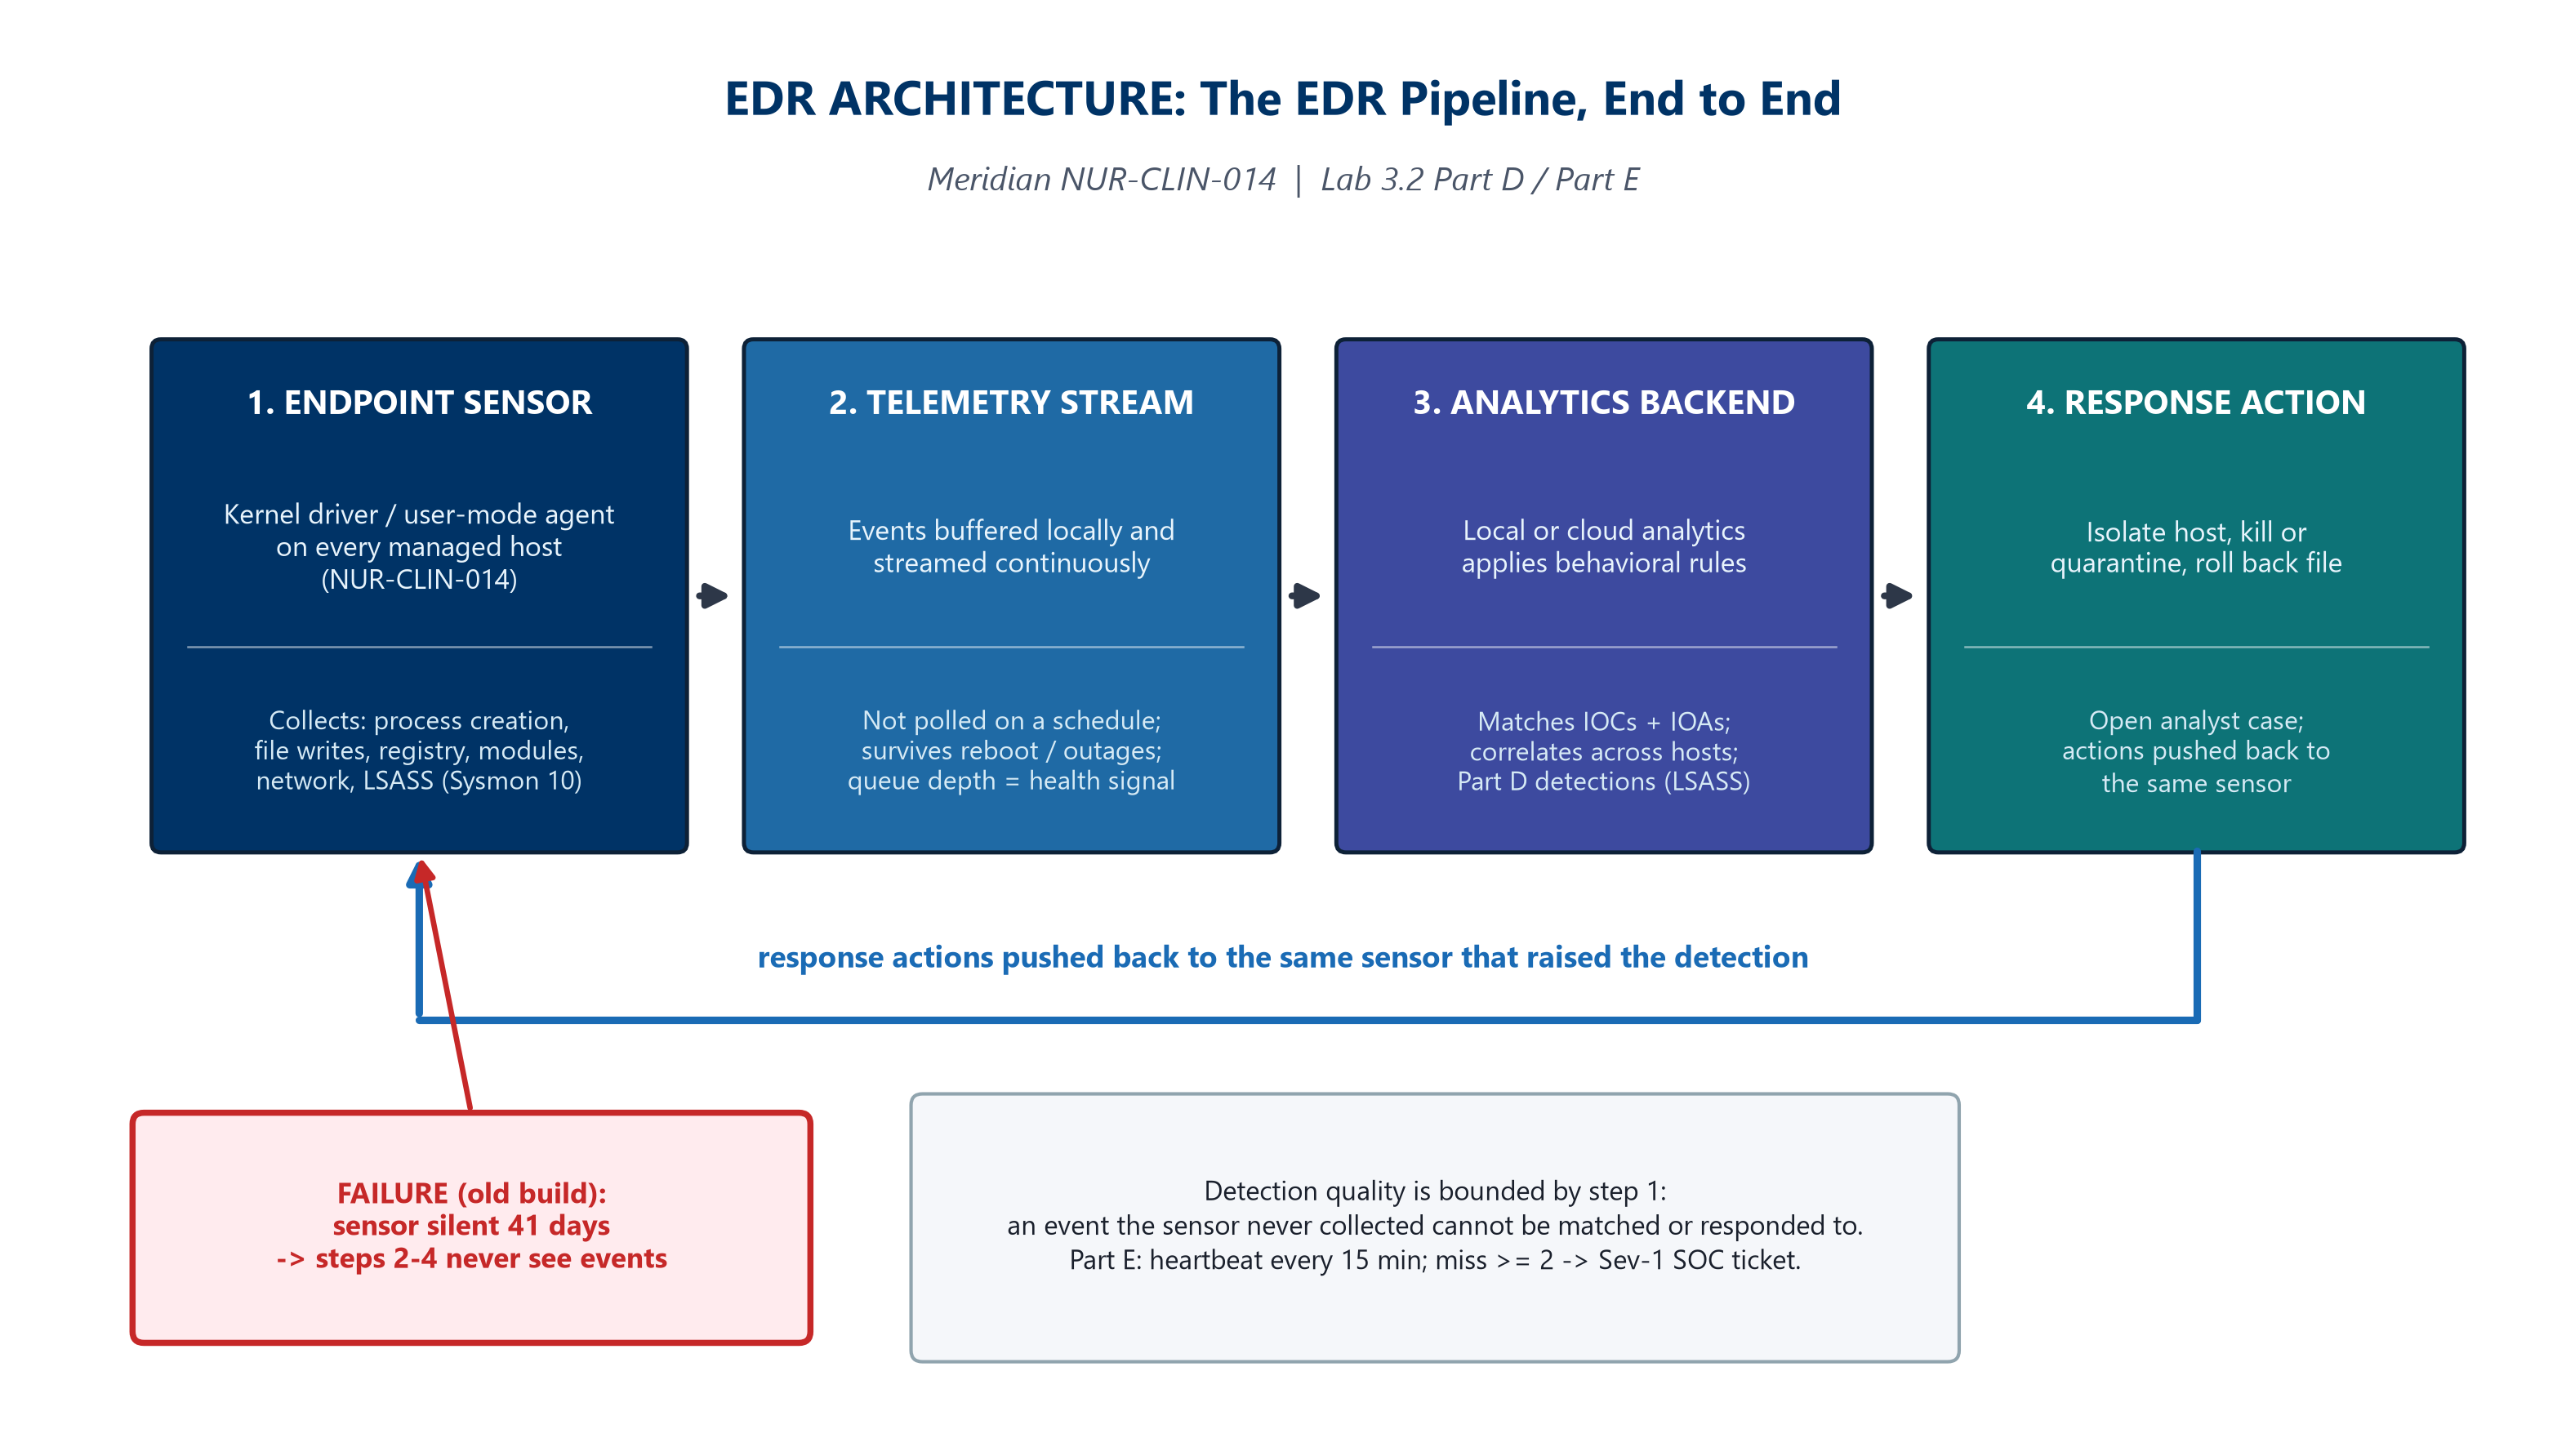
\includegraphics[width=0.98\textwidth]{figures/fig_edr_pipeline.png}
\caption{Author-created EDR pipeline for Meridian NUR-CLIN-014 (course four-stage architecture). The red callout marks the 41-day silent-sensor failure that left Steps~2--4 empty.}
\label{fig:edr}
\end{figure}

\noindent\textbf{EDR vs.\ XDR (scope for this lab).}
This rebuild instruments \textbf{EDR} on NUR-CLIN-014: host telemetry (processes, files, registry, local network, LSASS access) and host response (isolate, kill, quarantine). \textbf{XDR} would correlate endpoint plus network, email, identity, and cloud into one attack chain; valuable for Meridian later, but out of scope for a single rebuilt nurse station. The table below summarizes the difference.

\begingroup\labtablesetup
\rowcolors{2}{white}{tblrow}
\begin{tabularx}{\textwidth}{@{}>{\RaggedRight\arraybackslash}p{2.2cm} >{\RaggedRight\arraybackslash}X >{\RaggedRight\arraybackslash}X@{}}
\toprule
\rowcolor{tblhead}
\textcolor{white}{\textbf{Dimension}} &
\textcolor{white}{\textbf{EDR (this lab)}} &
\textcolor{white}{\textbf{XDR (future Meridian)}} \\
\midrule
\rowcolor{white}
Named & Gartner / Chuvakin $\sim$2013 & Gartner category $\sim$2020 \\
Telemetry scope & Endpoint: processes, files, registry/config, local network & Endpoint + network, email, identity, cloud workloads \\
Detection unit & Behavior on a single host, correlated across the fleet & Attack chain across different telemetry sources \\
Response surface & Host actions: isolate, kill, quarantine, roll back & Cross-source: disable account, quarantine message, isolate host \\
Best at catching & Local execution, persistence, credential access on a host & Chains that look benign in any one source and malicious in sequence \\
\bottomrule
\end{tabularx}
\endgroup

\subsection*{Step 5: Detection logic table}

\begingroup\labtablesetup
\rowcolors{2}{white}{tblrow}
\begin{tabularx}{\textwidth}{@{}>{\bfseries\centering\arraybackslash}p{0.55cm} >{\RaggedRight\arraybackslash}p{1.05cm} >{\RaggedRight\arraybackslash}p{2.15cm} >{\RaggedRight\arraybackslash}X >{\RaggedRight\arraybackslash}X@{}}
\toprule
\rowcolor{tblhead}
\textcolor{white}{\textbf{\#}} &
\textcolor{white}{\textbf{ID}} &
\textcolor{white}{\textbf{Telemetry Required}} &
\textcolor{white}{\textbf{Detection Logic}} &
\textcolor{white}{\textbf{Expected False Positive}} \\
\midrule
\rowcolor{white}
1 & T1547.001
  & Sysmon event 13/14 or registry audit 4657 + process image path
  & Alert when any process writes HKEY\_CURRENT\_USER (HKCU) / HKEY\_LOCAL\_MACHINE (HKLM) \texttt{...CurrentVersion\textbackslash Run} (or RunOnce) with ImagePath under \texttt{\%TEMP\%}, \texttt{Downloads}, or other user-writable path
  & Packaged software installer registering an updater during a change window. \\
2 & T1053.005
  & Task creation events (e.g., 4698) + task XML / action path
  & Alert on new scheduled task whose action path is user-writable OR author is a clinical interactive user (not SCCM/Intune service)
  & IT packaging task created by endpoint management during patch night. \\
3 & T1136.001
  & Security 4720 (account created) + 4732 (local group member add)
  & Alert on local account create outside Meridian naming convention OR any add to Administrators / Remote Desktop Users on NUR-CLIN hosts
  & Break-glass LAPS recovery workflow that creates a temporary admin (should be ticket-tagged). \\
4 & T1543.003
  & Service install 7045 / Sysmon service events + ImagePath
  & Alert when a new service starts automatically with ImagePath outside \texttt{Program Files} / Windows system directories, or runs as LocalSystem from a user-writable path
  & Vendor driver/service update pushed by approved imaging package. \\
5 & T1574.002
  & Image/library load events (Sysmon 7) with signer + path
  & Alert when an allowlisted clinical binary loads a DLL that is unsigned, newly written $<$24h, or from a user-writable directory
  & Vendor hotfixes that drop a new signed DLL next to the viewer (tune by publisher). \\
6 & T1070.001
  & Security 1102 (log cleared) + EDR sensor event
  & Critical alert on any Security log clear on clinical workstations; page SOC immediately
  & Rare, intentional log rotation by Tier~3 with change ticket (still should notify). \\
\bottomrule
\end{tabularx}
\endgroup

\noindent\textit{Additional high-signal rule (not one of the six mapped behaviors, but required by the old LSASS-dump finding on NUR-CLIN-014).}

\begingroup\labtablesetup
\begin{tabularx}{\textwidth}{@{}>{\bfseries\centering\arraybackslash}p{0.9cm} >{\RaggedRight\arraybackslash}p{2.0cm} >{\RaggedRight\arraybackslash}p{2.35cm} >{\RaggedRight\arraybackslash}X >{\RaggedRight\arraybackslash}X@{}}
\toprule
\rowcolor{tblhead}
\textcolor{white}{\textbf{\#}} &
\textcolor{white}{\textbf{Focus}} &
\textcolor{white}{\textbf{Telemetry Required}} &
\textcolor{white}{\textbf{Detection Logic}} &
\textcolor{white}{\textbf{Expected False Positive}} \\
\midrule
LSASS & Credential dump / LSASS memory access
  & Sysmon event~10 (ProcessAccess) to \texttt{lsass.exe}, or equivalent EDR handle-open telemetry (GrantedAccess, SourceImage, TargetImage)
  & Alert when any process other than known Microsoft / security products opens a handle to \texttt{lsass.exe} with read rights commonly used for credential dumping (e.g., \texttt{0x1010}, \texttt{0x1438}, or \texttt{PROCESS\_VM\_READ}); exclude allowlisted antivirus/EDR binaries by path and signature
  & Backup agents or security tools that legitimately read LSASS (must be inventory-allowlisted; unexpected callers still alert). \\
\bottomrule
\end{tabularx}
\endgroup

\subsection*{Step 6: Living off the land}

\textbf{Why allowlisting alone fails.}
Application allowlisting (WDAC) trusts Microsoft-signed system binaries. LOLBAS documents native utilities such as \texttt{certutil.exe}, \texttt{bitsadmin.exe}, and \texttt{mshta.exe} that are signed, required on a managed fleet, and can download or decode a second-stage payload. The binary is ``allowed,'' so the policy never blocks the abuse.

\textbf{Behavioral detection (not ``block certutil'').}
Alert when \texttt{certutil.exe} (or \texttt{bitsadmin.exe}) is created with a command line containing \texttt{-urlcache}, \texttt{-split}, \texttt{-decode}, or an http(s) URL, especially when the parent is a browser, Office app, or script host, and the child writes under a user-writable path. Fields: \texttt{OriginalFileName}/\texttt{Image}, \texttt{CommandLine}, \texttt{ParentImage}, \texttt{TargetFilename}, \texttt{User}, \texttt{UtcTime}.

\section*{5. Part E: The Silent Sensor}

\noindent\textbf{Where EDR does not help.}
Even a correct Part~D rule set fails in four cases the module names. Three of the four applied to NUR-CLIN-014 before anyone opened the host on Friday morning:

{\footnotesize
\begin{enumerate}\setlength{\itemsep}{0.25em}
\item \textbf{A sensor that is not reporting.} The most common failure is an absent detection (uninstalled, crashed, excluded, or stale agent), exactly the 41-day silence. Sensor health is a detection surface of its own (heartbeat below).
\item \textbf{Behavior indistinguishable from administration.} Remote execution, scheduled tasks, and service creation are also IT work. Detection quality depends on knowing ``normal'' for a shared nurse station (Part~D false-positive columns).
\item \textbf{Devices that cannot take an agent.} Lab~2.3 infusion pumps and other clinical embedded devices still need network segmentation and network detection; EDR on NUR-CLIN-014 does not cover them.
\item \textbf{Anything nobody triaged.} An alert in an unmonitored queue is the same as no detection. The pipeline ends with a human SOC analyst, not with the alert fire.
\end{enumerate}
}

\textbf{Sensor-health check.}
Measure EDR agent last-check-in timestamp and sensor service state every 5 minutes from the analytics backend. If a licensed Meridian clinical endpoint misses two consecutive 15-minute heartbeats (or reports \texttt{ServiceStopped}), raise a Sev-1 ticket to SOC Tier~1 and email the clinic IT on-call within 10 minutes. Owner: SOC Tier~1 with escalation to Endpoint Engineering.

\textbf{Which Step~5 detections still fire if the sensor is silent?}
None of them, including the additional LSASS handle-open rule. Every detection in Step~5 is written against telemetry the endpoint sensor must collect and transmit (Figure~\ref{fig:edr}). A silent agent means those events never reach the analytics backend, so registry, task, account, service, DLL-load, log-clear, and LSASS ProcessAccess rules cannot alert. That is why sensor health is a control of its own, not an afterthought.

\textbf{Residual risk the hardened build does not close.}
Physical shared-station risk remains: a clinician can walk away for under five minutes, or a malicious insider with a valid badge can operate inside WDAC/Credential Guard as a legitimate user. Hardening and EDR do not stop authorized-looking misuse of the EHR client. Closing that gap needs continuous session analytics (unusual chart access), camera/badge correlation for the corridor station, and stricter break-glass auditing, not more OS CIS checks alone. Credential Guard reduces LSASS dump value, but it does not stop an already-authorized clinician from misusing a valid session. For Meridian-wide attack chains that cross email/identity/cloud, EDR alone is also insufficient; that is the XDR gap noted in Part~D.

\section*{References}
\begin{hangparas}{1.5em}{1}
\refitem{cis}Center for Internet Security. (n.d.). \textit{CIS Benchmarks}. \url{https://www.cisecurity.org/cis-benchmarks}

\refitem{disa}Defense Information Systems Agency. (n.d.). \textit{Security Technical Implementation Guides (STIGs)}. \url{https://public.cyber.mil/stigs/}

\refitem{lolbas}LOLBAS Project. (n.d.). \textit{Living Off The Land Binaries, Scripts and Libraries}. \url{https://lolbas-project.github.io}

\refitem{mitre}MITRE Corporation. (n.d.). \textit{MITRE ATT\&CK Enterprise Matrix}. \url{https://attack.mitre.org}

\refitem{nist}National Institute of Standards and Technology. (2020). \textit{Security and privacy controls for information systems and organizations} (NIST SP 800-53 Rev.~5). \url{https://doi.org/10.6028/NIST.SP.800-53r5}
\end{hangparas}

\end{document}
